\documentclass[10pt, aspectratio=169, compress]{beamer}
\usetheme[progressbar=frame title, numbering=fraction]{metropolis}      % Use metropolis theme 
\setbeamertemplate{section in toc}[sections numbered]
\setbeamertemplate{subsection in toc}[subsections numbered]
\useoutertheme[subsection=false]{miniframes}
\setbeamercolor{section in head/foot}{fg=white, bg=mDarkTeal}
\setbeamercolor{background canvas}{bg=white}
\setbeamerfont{section in head/foot}{series=\bfseries}

\usefonttheme[onlymath]{serif}
\usepackage{amsmath}
\usepackage{remreset}
\usepackage{ragged2e}
\usepackage{booktabs}
\usepackage{makecell}
\usepackage{float}
\usepackage{subfig}
\usepackage{tikz}
\usetikzlibrary{positioning,calc,trees}
\usepackage[flushleft]{threeparttable}	% 3 part table 
\usepackage[justification=centering]{caption}
\captionsetup{skip=0pt}
\graphicspath{{./fig/}}

\makeatletter
\let\beamer@writeslidentry@miniframeson=\beamer@writeslidentry
\def\beamer@writeslidentry@miniframesoff{%
	\expandafter\beamer@ifempty\expandafter{\beamer@framestartpage}{}% does not happen normally
	{%else
		% removed \addtocontents commands
		\clearpage\beamer@notesactions%
	}
}
\newcommand*{\miniframeson}{\let\beamer@writeslidentry=\beamer@writeslidentry@miniframeson}
\newcommand*{\miniframesoff}{\let\beamer@writeslidentry=\beamer@writeslidentry@miniframesoff}
\beamer@compresstrue
\makeatother

%==============================================================
% Title Page
%==============================================================
%Information to be included in the title page:
\title{Construcción de Datos}
\subtitle{Manejo y limpieza}
\author{Rony Rodriguez-Ramírez} 
\institute{LAMBDA}
\titlegraphic{\hfill
\includegraphics[height=1.5cm]{dime}}
\date{\today}
%==============================================================
\begin{document}
%------------------------------------------------	
\begin{frame}[plain]
	\maketitle 
\end{frame}
%------------------------------------------------
\section{Construcción de Datos}
%-----------------------------------------------
\subsection{Construcción de Datos}
%-----------------------------------------------
\begin{frame}{Desglose de tareas de trabajo de datos}
	\begin{itemize}
		\item Dividimos el proceso de trabajo de datos en cuatro etapas:
		\begin{enumerate}
			\item De-identificación
			\item Limpieza de datos
			\item Construcción de variables
			\item Análisis de datos
		\end{enumerate}
		\item Cada una de estas etapas tiene entradas y salidas bien definidas.
		\item Para cada etapa, debe haber una carpeta de códigos y un conjunto de datos correspondiente
		\item Los nombres de códigos, conjuntos de datos y salidas para cada etapa deben ser consistentes
		\item El código, los datos y los resultados de cada una de estas etapas deben pasar por al menos una ronda de revisión de código.
	\end{itemize}
\end{frame}
%-----------------------------------------------
\begin{frame}{Recopilación e importación de datos.}
	\begin{itemize}
		\item Para esta presentación, asumiremos que ya ha recopilado e importado sus datos.
		\item En la práctica, sin embargo, la limpieza de datos comienza antes de que termine la recopilación de datos
		\item Las siguientes tareas de recopilación de datos que, cuando se realizan correctamente, hacen que la limpieza de datos sea mucho más fácil:
		\begin{enumerate}
			\item Programación de encuestas
			\item Monitoreo de calidad de datos
			\item Importación de datos
		\end{enumerate}
	\end{itemize}
\end{frame}
%-----------------------------------------------
%-----------------------------------------------
\section{De-identificación}
\subsection{De-identificación}
%-----------------------------------------------
\begin{frame}[t]{Input: Los datos sin procesar (raw data)}
	\begin{itemize}
		\item Contiene solo información recibida directamente del campo.
		\item Los archivos de datos sin procesar deben almacenarse en la carpeta de datos sin procesar exactamente como se recibieron.
		\item Tenga en cuenta cómo y dónde se almacenan: no se pueden volver a crear y casi siempre contienen datos confidenciales
		\item Los archivos de datos sin procesar nunca deben editarse directamente
		\item Si los datos sin procesar contienen información confidencial, deben estar encriptados
		\item Asegúrese de tener una copia de seguridad de los datos sin procesar (con suerte, nunca necesitará usarlos)
	\end{itemize}
\end{frame}
%-----------------------------------------------
\begin{frame}[t]{Output: Datos de-idenficados}
	\begin{itemize}
		\item Versión de trabajo del conjunto de datos que se puede compartir dentro del equipo de investigación sin riesgo
		\item Contiene solo información recibida directamente del campo
		\item No contiene identificadores directos
		\item No es necesariamente anónimo
		\item Por lo general, la desidentificación no debe afectar la usabilidad de los datos.
	\end{itemize}
\end{frame}
%-----------------------------------------------
\begin{frame}[t]{Identificar identificadores directos}
	\begin{itemize}
		\item Lo primero que necesita para de-identificar los datos es una lista de todos los identificadores directos en el conjunto de datos
		\item Idealmente, todas las variables potencialmente identificables se marcan durante el diseño del cuestionario.
		\item Herramientas útiles:
		\begin{itemize}
			\item \texttt{Escaneo PII} de JPAL
			\item \texttt{SdcMicro} del Banco Mundial
			\item \texttt{Iecodebook} de DIME Analytics
		\end{itemize}
	\end{itemize}
\end{frame}
%-----------------------------------------------
\begin{frame}[t]{Eliminar identificadores directos}
	Una vez que tenga una lista de todos los identificadores directos, para cada uno de ellos, pregúntese (y el plan de preanálisis):
	\begin{enumerate}
		\item ¿Será necesaria esta variable para el análisis?
	\begin{itemize}
		\item Si la respuesta es no, simplemente suéltela
		\item No tenga miedo de descartar demasiadas variables: siempre puede recuperarlas (pero no puede deshacer una fuga de datos)
	\end{itemize}
	\item ¿Puedo codificar o construir una variable que enmascara la PII?
	\end{enumerate}
\end{frame}
%-----------------------------------------------
\section{Data cleaning}
\subsection{Data cleaning}
%-----------------------------------------------
\begin{frame}[t]{Data cleaning}
	Durante la limpieza de datos, observará cuidadosamente cada variable en su conjunto de datos. Los objetivos de este proceso son:
	\begin{itemize}
	\item Hacer que el conjunto de datos sea fácilmente utilizable y comprensible.
	\item Documentar puntos de datos individuales y patrones que pueden sesgar el análisis.
	\end{itemize}
\end{frame}
%-----------------------------------------------
\begin{frame}[t]{Introducción}
	\begin{itemize}
		\item La limpieza es probablemente la tarea de trabajo de datos que consume más tiempo, y se sentirá tentado a omitirla.
		\item Sin embargo, este es el momento cuando realmente conozca sus datos.
		\item Explore su conjunto de datos usando tabulaciones (tab), summ y diagramas (plots) descriptivos.
		\item Conocer bien su conjunto de datos permitirá hacer análisis
		\item Limpiar bien sus datos le ahorrará tiempo.
	\end{itemize}
\end{frame}
%-----------------------------------------------
\begin{frame}{Output: Una base de datos limpia}
	\begin{center}
		¿Qué creen que nos referimos con una base de datos limpia? 
	\end{center}
\end{frame}
%-----------------------------------------------
\begin{frame}[t]{Output: Una base de datos limpia}
	\begin{itemize}
		\item Al final de este proceso, debe tener un conjunto de datos que sea esencialmente el mismo que descargó del servidor.
		\item La principal diferencia es que el conjunto de datos limpios debería ser más fácil de entender para cualquiera que lo abra por primera vez.
	\end{itemize}
\end{frame}
%-----------------------------------------------
\begin{frame}[t]{Output: Una base de datos limpia}
	\begin{itemize}
		\item También debe remontarse fácilmente al instrumento de encuesta.
		\item Por lo general, se creará un conjunto de datos limpios para cada fuente de datos o instrumento de encuesta.
		\item El conjunto de datos limpios y no identificados, más la documentación que lo respalda, son los primeros datos de salida de su proyecto: un conjunto de datos publicable.
	\end{itemize}
\end{frame}
%-----------------------------------------------
\begin{frame}[t]{Output: Documentación}
	Algunas piezas de documentación deben acompañar al conjunto de datos limpios:
	\begin{itemize}
		\item Un diccionario de variables, o libro de códigos, que enumera detalles sobre las variables en el conjunto de datos.
		\item Los instrumentos utilizados para recopilar los datos.
		\item Un registro completo de las correcciones realizadas a los datos sin procesar, incluida una explicación cuidadosa sobre el proceso de toma de decisiones involucrado
		\item Un informe que documente cualquier irregularidad adicional y patrones de distribución encontrados en los datos.
	\end{itemize}
\end{frame}
%-----------------------------------------------
\begin{frame}[t]{Unique ID}
	\begin{itemize}
		\item Lo primero que desea buscar cada vez que abre un nuevo conjunto de datos por primera vez es
		\begin{enumerate}
			\item Unidad de observación.
			\item Identificación única y totalmente variable de identificación.
		\end{enumerate}
		\item Antes de separar los datos identificables de los no identificados, asegúrese de saber cómo cruzar ambos utilizando la ID única
	\end{itemize}
\end{frame}
%-----------------------------------------------
\begin{frame}[t]{Propiedades deseables de una variable ID}
	\begin{enumerate}
		\item Identificación única
		\item Totalmente identificable
		\item Anónimo
		\item Constante dentro de un proyecto
	\end{enumerate}
	¿Cómo probaría si una variable se identifica de manera única y completa?
\end{frame}
%-----------------------------------------------
\begin{frame}[t]{Unique ID}
	Comandos para probar que la variable en Stata:
	\begin{itemize}
		\item \texttt{isid}
		\item \texttt{codebook}
	\end{itemize}
\end{frame}
%-----------------------------------------------
\begin{frame}{¿Cuál es la unidad de observación?}
	\begin{figure}[H]
		\centering
		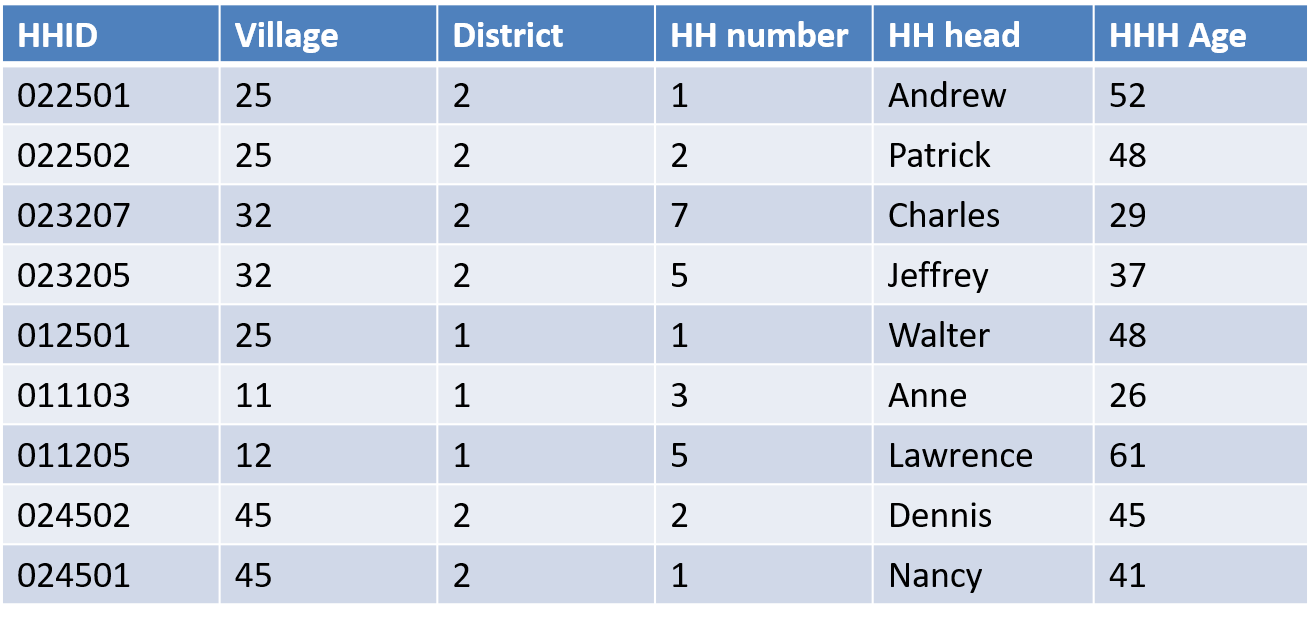
\includegraphics[width=0.8\textwidth]{hh_data.png}
	\end{figure}	
\end{frame}
%-----------------------------------------------
\begin{frame}{¿Cuál es la unidad de observación?}
	\begin{figure}[H]
		\centering
		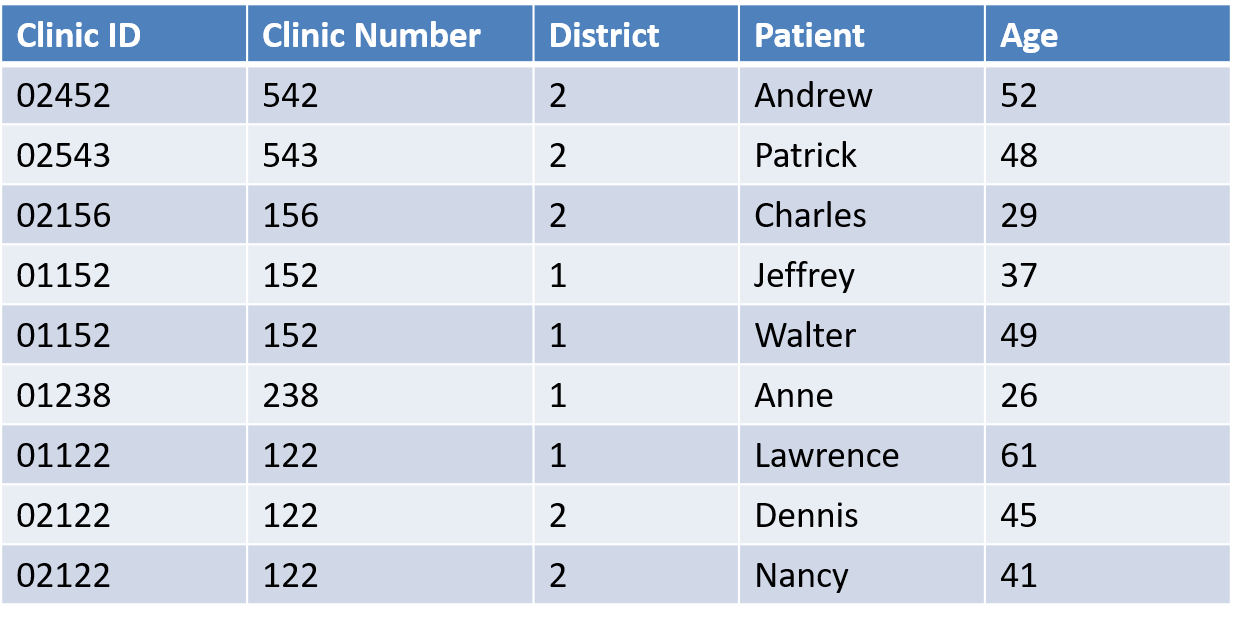
\includegraphics[width=0.8\textwidth]{clinic_data.png}
	\end{figure}	
\end{frame}
%-----------------------------------------------
\begin{frame}[t]{Usando \texttt{iefieldkit} para resolver entradas duplicadas}
	\begin{itemize}
		\item El comando \texttt{ieduplicates} ayuda a identificar y resolver duplicados en datos de encuestas sin procesar.
		\item El comando genera un informe de todas las entradas duplicadas de una variable (en Excel) y elimina los duplicados del conjunto de datos hasta que se resuelven.
		\item El informe de Excel se utiliza para documentar los casos de entrevistas duplicadas y cómo se resolvieron.
	\end{itemize}
\end{frame}
%-----------------------------------------------
\begin{frame}[t]{Correcciones en el ingreso de datos}	
	\begin{itemize}
		\item Durante la recopilación de datos, particularmente durante la recopilación de datos primarios, es probable que los enumeradores y supervisores informen los problemas
		\item Durante el monitoreo de la calidad de los datos, es probable que también identifique los problemas que deben abordarse
		\item Ejemplos de eso son errores tipográficos, identificaciones incorrectas y nuevas encuestas
		\item Es importante registrar todos estos problemas y las comunicaciones sobre ellos.
		\item Este es el único caso, aparte de las ID duplicadas, cuando cambiará los puntos de datos durante la limpieza de datos
		\item \textbf{Haga todas las correcciones en un do file}, no manualmente, y recuerde documentar de dónde proviene la información
	\end{itemize}
\end{frame}
%-----------------------------------------------
\section{Crear un conjunto de datos anotados}
\subsection{Crear un conjunto de datos anotados}
%-----------------------------------------------
\begin{frame}[t]{Label variables (etiquetas)}
	Al limpiar un conjunto de datos, debe asegurarse de que todas las variables estén correctamente etiquetadas, de modo que sea fácil entender qué representa cada variable:
	\begin{itemize}
		\item Verifique que todas las variables tengan etiquetas de variables.
		\item Las etiquetas de las variables deben explicar qué es la variable y, si ese es el caso, en qué unidad está.
		\item Las etiquetas no pueden tener más de 80 caracteres.
	\end{itemize}
\end{frame}
%-----------------------------------------------
\begin{frame}[t]{Cifrando variables (\texttt{encode})}
	\begin{itemize}
		\item La base de datos limpia no debe contener variables de cadena (string variables, i.e., \texttt{texto}), excepto
		\begin{itemize}
			\item Nombres propios que no son categorías
			\item Dígitos con ceros a la izquierda o ID largos (más de 15 dígitos)
		\end{itemize}
		\item Eso significa que las variables de cadena (string) deben transformarse en variables categóricas o factores etiquetados.
		\item Tenga en cuenta las preguntas abiertas: presentan un riesgo mucho mayor de divulgación estadística.
		\item Verifique que todas las variables categóricas tengan value labels (etiquetadas con valor).
	\end{itemize}
\end{frame}
%-----------------------------------------------
\begin{frame}[t]{Encoding variables en Stata}
	\begin{itemize}
		\item En Stata, la mejor práctica es usar la codificación tanto con la etiqueta (\texttt{label}) como con las opciones de no extensión (\texttt{noextend}).
		\item Otros comandos útiles: \texttt{label define, label value, label dir, label list, labelbook}.
		\item Si usó SurveyCTO, usó la etiqueta de columna: stata y los datos se importaron correctamente, este paso puede no ser necesario. 
	\end{itemize}

	\begin{center}
		Ejemplo: \texttt{encode dist name, generate(dist id) label(district) noextend}
	\end{center}
\end{frame}
%-----------------------------------------------
\begin{frame}[t]{Extended missing values}
	\begin{itemize}
		\item Durante la recopilación de datos primarios, use códigos como -88, -9, -777 para representar diferentes razones de datos faltantes, como "no sabe", "se negó a responder", etc.
		\item Es necesario eliminar estos valores, ya que de lo contrario sesgarán los medios.
		\item Si los cambiamos a todos como perdidos, perderemos información.
		\item Use valores perdidos extendidos para mantener la información, pero aún así le dice a Stata que los trate como perdidos.
	\end{itemize}
\end{frame}
%-----------------------------------------------
\begin{frame}[t]{Extended missings values en Stata}
	\begin{itemize}
		\item El missing value  regular en Stata es: .
		\item Use missing values extendidos para representar la misma razón de la falta de datos en todo el proyecto:
		\begin{itemize}
			\item .d = "No sé / Don't know"
			\item .r = "Se negó a responder / Refused to answer"
			\item .s = "Saltado / Skipped"
		\end{itemize}
		\item Los valores perdidos también se pueden etiquetar.
	\end{itemize}
\end{frame}
%-----------------------------------------------
\begin{frame}[t]{Extended missings values en Stata}
	\begin{itemize}
		\item Para Stata, números $ < . < .a < .b < .c < \cdot < .z $
		\item Así que reemplace esto:
		\linebreak
		\texttt{sum HH\_ingreso if employment != .}
		\linebreak
		Con esto:
		\linebreak
		\texttt{sum HH\_ingreso if employment < .}
		\linebreak
		\texttt{sum HH\_ingreso if !missing(employment)}
	\end{itemize}
\end{frame}
%-----------------------------------------------
\begin{frame}[t]{Renombrando variables}
	\begin{itemize}
		\item No cambie los nombres de las variables que provienen de una encuesta, incluso si no le gustan las convenciones de nomenclatura utilizadas en el cuestionario.
		\item Cambiar el nombre de las variables hará que sea más difícil encontrar la correspondencia entre las variables y las preguntas de la encuesta.
	\end{itemize}
	Artículo sobre el nombre de las variables en \href{https://medium.com/@janschenk/variable-names-in-survey-research-a18429d2d4d8}{\color{blue}{Medium}}
\end{frame}
%-----------------------------------------------
\begin{frame}[t]{Usando \texttt{iefieldkit para anotar una base de datos}}
	\begin{itemize}
		\item El comando iecodebook le ayuda a realizar la mayoría de las tareas descritas anteriormente (con la excepción de la codificación)
		\item El comando genera (en Excel) una lista de todas las variables en el conjunto de datos y sus etiquetas, y les aplica los cambios para simplificar el proceso.
		\item El informe de Excel se utiliza para documentar las modificaciones realizadas en el conjunto de datos durante la limpieza.
	\end{itemize}	
\end{frame}
%-----------------------------------------------
\section{Otras tareas en la limpieza de datos}
\subsection{Otras raeas en la limpieza de datos}
%-----------------------------------------------
\begin{frame}[t]{Recategorizando valores listado como "Otros"}
	\begin{itemize}
		\item Las variables categóricas generalmente tienen una opción abierta "otro, especificar" que se guarda como una cadena
		\item Las respuestas que aparecen con frecuencia en la pregunta abierta se pueden incluir como una nueva categoría en la variable categórica
		\item Eso generalmente se realiza durante el piloto o las comprobaciones de alta frecuencia, pero es posible que aún se omitan categorías relevantes
	\end{itemize}
\end{frame}
%-----------------------------------------------
\begin{frame}[t]{Eliminar variables de la encuesta}
	\begin{itemize}
		\item \item Algunas variables se crean para ser utilizadas dentro de la encuesta y para las comprobaciones de la encuesta.
		\item Ese es el caso de la mayoría de los campos de cálculo, así como las notas y las variables de duración.
		\item Las variables que no forman parte del cuestionario en sí pueden eliminarse del conjunto de datos limpio.
	\end{itemize}
\end{frame}
%-----------------------------------------------
\begin{frame}[t]{Ordenar variables}
	\begin{itemize}
		\item Se recomienda que las variables en el conjunto de datos final sigan un cierto orden como en el cuestionario
		\item Si creó nuevas variables durante la limpieza de datos, por ejemplo, para cambiar los códigos de la lista, probablemente estarán fuera de servicio
		\item Es posible que desee reordenar esas variables para que el conjunto de datos sea más fácil de leer y comparar con el cuestionario.
	\end{itemize}
\end{frame}
%-----------------------------------------------
\section{Convenciones para guardar archivos}
\subsection{Convenciones para guardar archivos}
%-----------------------------------------------
\begin{frame}[t]{Guardando archivos}
	\begin{itemize}
		\item Durante el proceso de limpieza de datos, es posible que haya guardado varios archivos intermedios, por ejemplo, si limpió módulos largos por separado para que su código sea más legible.
		\item Después de limpiar sus datos y fusionarlos nuevamente, querrá guardar un conjunto de datos limpios final, que contenga todas las variables de su encuesta.
	\end{itemize}
\end{frame}
%-----------------------------------------------
\begin{frame}[t]{Guardando archivos}
	\begin{itemize}
		\item Este nuevo conjunto de datos probablemente será bastante pesado. Use \texttt{compress} para guardar sus variables en el formato más económico (i.e., tamaño).
		\item A menudo es deseable guardar su conjunto de datos en una versión anterior de Stata, por lo que otros miembros de su equipo no tendrán conflictos de versión. Para hacer esto, use \texttt{saveold}.
	\end{itemize}
\end{frame}
%-----------------------------------------------
\begin{frame}[t]{Nombrando archivos}
	\begin{itemize}
		\item Asegúrese de que todos los archivos de salida, conjuntos de datos y otros estén etiquetados de forma clara y única, es decir: "desc\_stats\_tmt\_only.xls" "input\_plan\_adm\_data.dta"
		\item A menudo es deseable tener los nombres de sus conjuntos de datos y archivos do vinculados, por lo que es fácil entender qué archivos do están creando qué conjunto de datos, como "merge.do" y "merged.dta" o "cleaning.do" y "clean.dta".
		\item No utilice \_v1, \_v2, etc. para ningún archivo final. Esto conduce a errores en los archivos do que dependen de estos archivos cuando se agrega una nueva versión.
		\item Está bien usar \_v1, \_v2, etc. para versiones antiguas de archivos si realmente necesita mantener un archivo
	\end{itemize}
\end{frame}
%==============================================================
% Stata TIME
%==============================================================
\miniframesoff 	

\begin{frame}[plain, noframenumbering]
	\begin{center}
	\LARGE STATA TIME
		\begin{figure}[H]
			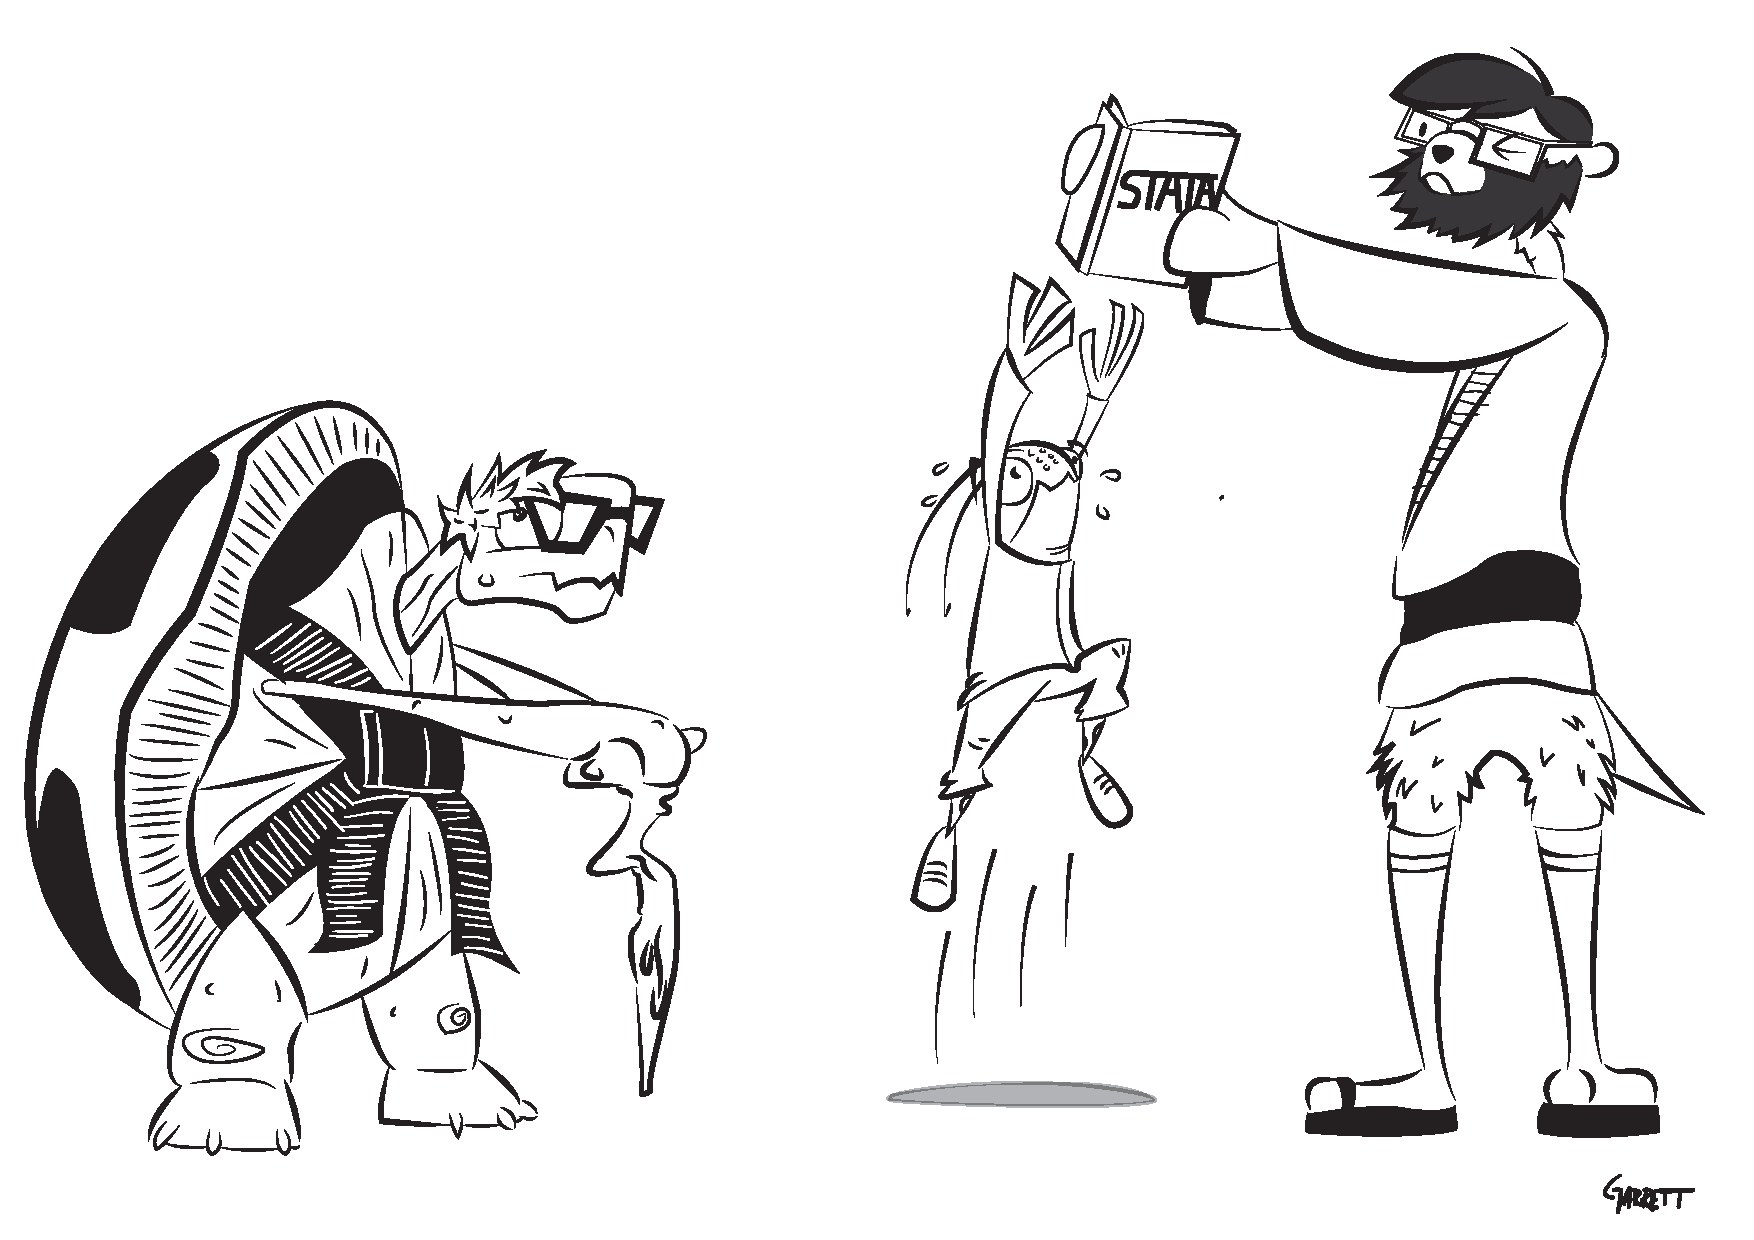
\includegraphics[width=0.57\textwidth]{stata.pdf}
		\end{figure}
	\end{center}
\end{frame}
%==============================================================
% END
%==============================================================	
\begin{frame}[plain, standout]
	Nos vemos mañana.
\end{frame}
%-----------------------------------------------
\end{document}		
